\documentclass[output=paper]{LSP/langsci} 
\ChapterDOI{10.5281/zenodo.2563690}
\author{Lourens de Vries\affiliation{Vrije Universiteit Amsterdam}}
\title{Online and offline bridging constructions in Korowai} 
%%%\epigram{Change epigram in chapters/01.tex or remove it there }

\abstract{Korowai has two main types of bridging constructions, recapitulative linkage  (also known as ``tail-head linkage'') and summary linkage with generic verbs of doing, each with two subtypes that follow from the grammatical distinction between chained and adverbial or thematic types of clause combining. Recapitulative linkage with chained, switch reference marked clauses is by the far the most frequent type of bridging construction. It has three functions. First, a processual function, to give the speaker and addressee a processing pause in between two often lengthy clause chains. Second, it creates chains of clause chains, so called chaining paragraphs. The third function is to enable the speaker  to  continue  referential tracking in the transition from one clause chain to the next.  Recapitulative linkage with thematic subordinate clauses shares the processual function wih the chained type but it signals discourse discontinuity:  it disrupts the event and participant lines and the speaker goes off the event line. Summary linkage allows speakers to be less specific in the scope of their anaphoric linkage, not necessarily taking the final clause of the previous sentence as their reference clause.}
\maketitle


\begin{document}\label{ch:7}

\section{Introduction} 
\label{Devsec:Introduction}
\ili{Korowai} is a Papuan language of the Greater Awyu family spoken by around 4000 persons in the area between the upper Becking and Eilanden Rivers and east of the headwaters of the Becking River in Indonesian West Papua, in the Boven-Digul regency (\citealt{enk97}; \citealt{devries.2012}). \ili{Korowai} is a synthetic language, with agglutinating morphology and some fusion. Verb morphology is suffixing, but \ili{Korowai} has a negation circumfix. Verbal affixes mark mood, modality, tense, aspect, negation, person and number of the subject (S and A) and \isi{switch reference}. The opposition Realis and Irrealis is central to the verb system, and tense is dependent on the Realis and Irrealis distinction, as in all Greater Awyu languages (\citealt{wester14}). \ili{Korowai} nouns have little morphology. Nouns may take possessive prefixes. Only kinship nouns have plural suffixes.

To understand \ili{Korowai} bridging constructions and some of the grammatical terminology used in Papuan linguistics, it is crucial to introduce three major \ili{Korowai} clause linkage patterns, conjoining, adverbial clause combining and chaining. The first two types are cross-linguistically common; the last type, \isi{clause chaining}, occurs in many Papuan language families (especially in the cluster of families called the Trans New Guinea group) but is cross-linguistically less common. Conjoining of clauses (asyndetic or with coordinating conjunctions) is a relatively infrequent type of clause linkage (compared to \isi{clause chaining}) in \ili{Korowai}. Conjoining linkage joins two independent clauses of equal syntactic status, as in (\ref{Devex:01ab}):

\begin{exe}
\ex \label{Devex:01ab}
\gll if-e=xa abül=efè xoŋgél=xayan waf-e=xa abül=efè be-xoŋgé-tebo-da\\
this-\textsc{tr=conn} man=\textsc{top}	big=very that-\textsc{tr=conn}	man=\textsc{top} \textsc{neg}-big-be[\textsc{non1.sg.rls}]-\textsc{neg}\\
\glt \sqt{This man is bigger than that man.}
(lit. `This man is very big, that man is not big.') \citep[][71]{enk97}\\
\end{exe}

\noindent
When coordinating conjunctions are absent, as in (\ref{Devex:01ab}), it is only the intonational integration of the two member clauses under a joint contour that distinguishes a single conjoined sentence from two juxtaposed sentences. 

Adverbial clause combining, with various subtypes, occurs when a clause functions as a peripheral argument of another clause or when a clause functions as an extra-clausal theme that precedes a clause with which it has a pragmatic relation of relevance. Adverbial (or better: thematic) clauses are marked by the general subordinator =\textit{xa} and present information that the speaker wants the addressee to take for granted, as the given theme for the following assertion. The semantic function of the thematic clause may be explicitly marked as in (\ref{Devex:11b}) but is often left implicit. The informational status of the theme clause is optionally but frequently marked by the \isi{topic} clitic \textit{=efè} (with allomorphs \textit{=fefè} and \textit{=fè}). There is an example of a thematic clause in (\ref{Devex:02}) \textit{bul‑mexo=xa=fefè} `given that he slaughtered'. The term theme is used here in the sense of \citet{Heeschen98} to denote thematization strategies found in many Papuan languages where thematic noun phrases or thematic clauses are marked in a loose sense as relevant domains or themes for the information that follows \citep[][814--816]{devries.2006}.


\begin{exe}
\ex \label{Devex:02}
\gll \textit{Faül} \textit{dadü-ai=to=fexo} Faül ül-nè bul-mexo=xa=fefè Faül ba-nggolol yaüya=pé fe-nè	fu=to=fexo méan dadü-ai méan ül-nè bul-fo=xa=fè méan-manop-yabén=tompexo di-béa-mo=daxu i=fexo wolaxip wolaxif=exa Faül müfe‑xolol di \textit{lamé‑abo‑lu}\\
Faül swim-go.down[\textsc{non1.sg.rls}]=\textsc{ds}=\textsc{conn} Faül kill-\textsc{ss} slaughter-do[\textsc{non1.sg.rls}]=\textsc{conn}=\textsc{top} Faül chest-bone under=\textsc{loc} get-\textsc{ss} put[\textsc{non1.sg.rls}]=\textsc{ds}=\textsc{conn} dog swim-go.down[\textsc{non1.sg.rls}] dog kill-\textsc{ss} slaughter‑make[\textsc{non1.sg.rls}]=conn=top dog-chest-fat=\textsc{emph} get.out-rub-do[\textsc{non1.sg.rls}]=\textsc{ss} here=at heaven heaven=\textsc{conn} Faül back‑bone cut.\textsc{ss} dance‑chase‑move.up[\textsc{non1.sg.rls}]\\
\glt \sqt{Faül came swimming downstream, after having killed and slaughtered Faül, he put its chest bone part beneath, and its back bone part he placed towards the sky and having killed and  butchered a dog that came swimming downstream, he cut out the fat of the dog's chest and greased  the back bone part of Faül and he chased it upward in a hurry.} \citep[][165]{enk97}\\
\end{exe}

Clause chaining combines \isi{switch reference} marked clauses into often long sentences (called clause chains in Papuan linguistics) that end in a \isi{final clause} with an independent verb form. That verb in the \isi{final clause} of the chain has tense and mood scope over the preceding sentence. In canonical \isi{clause chaining} languages of New Guinea, the verb types used in the final clauses are different from the verb types used in non-final or medial clauses. On the one hand, medial verb types  cannot express the full range of tense, mood, person and number distinctions that final verbs encode, on the other hand medial verbs have slots for categories of interclausal relations absent in final verbs, namely \isi{switch reference} (Same Subject or Different Subject in next clause of the chain) and temporality (Sequence versus Simultaneity relations between the events of two adjacent clauses in the chain).

Like other Greater Awyu languages, \ili{Korowai} is a non-canonical chaining language compared to many other languages of the Trans New Guinea type because its dedicated medial verb morphology is weakly developed \citep{devries.2010}. The only dedicated medial verb type is the Same Subject verb that consists of a verb stem plus an optional Same Subject suffix. There are also no dedicated Different Subject medial verbs in \ili{Korowai} as found in more canonical Papuan \isi{clause chaining} languages. Instead, \ili{Korowai} uses clauses with fully inflected independent verbs (the type that must be used in the final clauses of sentences) with \isi{switch reference} clitics. This is the set of \isi{switch reference} conjunctions in  \ili{Korowai} \citep[][109]{enk97}: 

%vvvvvvvvvvvvvvvvvvvvgggggggggggggggggggggggggg remove too much spacing
\begin{description}
\item[=\textit{do(n)}] 		`different subject'
 		\item[=\textit{daxu(l)}] 	`same subject'
     	\item[=\textit{aŋgu}]			`same subject/intentional'
     	\item[=\textit{(le)lexu}]	`different subject/irrealis/anteriority'
\end{description}
		
\noindent
Chaining is by far the most used type of clause linkage in the \ili{Korowai} texts available to us and chained clauses are strongly associated with \isi{thematic continuity} within a \isi{clause chain}. 

Thematic adverbial clauses are associated with discontinuity, when speakers discontinue the flow of the main event and participant lines, either within a sentence, or in the transition from one sentence to another, for special reasons: to present background information, to mention circumstances that formed the cause or reason for an event of the main line, or to start a new paragraph (\citealt[][337, 363]{farr99}; \citealt[][373]{devries.2005}). A typical \ili{Korowai} \isi{clause chain}, as in (\ref{Devex:02}), contains \isi{switch reference} marked chained clauses, with medial verbs (for example \textit{ül‑nè}) and with \isi{switch reference} marked independent verb forms (\textit{dadü-ai=tofexo}). The \isi{final clause} of the \isi{clause chain} (\ref{Devex:02}) contains the independent verb \textit{lamé‑abo‑lu}. Within  sentence  (\ref{Devex:02}), we find two thematic clauses \textit{bul‑fo=xa=fè} and \textit{bul‑mexo=xa=fefè}. They are not \isi{switch reference} marked but they are marked for their informational role as themes by the \isi{topic} marker \textit{=(fe)fè}. The \isi{event line} of (\ref{Devex:02}) is twice disrupted by these thematic clauses. The idiomatic translation of the first thematic clause reads ‘after he had slaughtered’ but the semantic functions that thematic clauses have (temporal, locative and so on) are usually left to be contextually inferred, and this is also the case in (\ref{Devex:02}). A translation closer to the sense of the first thematic clause in (\ref{Devex:02}) would be `given that he slaughtered'. 

Such generic thematic clauses are very versatile in terms of the wide range of interpretations that addressees may contextually infer. Thematic clause combining occurs in many Papuan languages with similar functions and may often be translated idiomatically with adverbial or relative clauses in \ili{English} (\citealt{haiman.1978,reesink94,Heeschen98}; \citealt[][201]{foley86}). Consider example (\ref{Devex:03}):

\begin{exe}
\ex \label{Devex:03}
\gll Wa gol ülme-tél=exa=fè noxu-gol\\	
that pig  kill-\textsc{non1.pl}[\textsc{rls}]=\textsc{conn}=\textsc{top} our-pig\\
\glt \sqt{The pig that they killed, is our pig.} (`given that they killed the pig, it is our pig').\\
\end{exe}

If the assertion had been `we are angry' instead of \textit{noxu-gol} `our pig', the interpretation would have been `because they killed the pig, we are angry' \citep[][826]{devries.2006}. \ili{Korowai} has two main types of bridging constructions, \isi{recapitulative linkage} (\refsec{Devrecap.link})
and \isi{summary linkage} (\refsec{Devsumm.link}). Both types each have two subtypes that follow from the two types of clause linkage illustrated in (\ref{Devex:02}) and (\ref{Devex:03}), \isi{switch reference} marked chaining linkage and \textit{=xa} marked thematic subordinate linkage. The terms bridging constructions, \isi{recapitulative linkage}, \isi{summary linkage}, reference clause and bridging clause are used in this article as defined in the introductory chapter of this volume.


\section{Recapitulative linkage} 
\label{Devrecap.link}
There are two subtypes of \isi{recapitulative linkage} (formerly, tail-head linkage) in \ili{Korowai} \citep[][372--374]{devries.2005}. In the first type the bridging clause takes the form of a \isi{switch reference} marked chained clause. The bridging clause of the second type is a thematic clause marked with the clitic \textit{=xa} and optionally marked by the \isi{topic} marker \textit{=(fe)fè}. 

\subsection{Recapitulative linkage with chained clauses} 
\label{Devrecap.link.chained}
Recapitulative linkage with \isi{switch reference} marked bridging clauses is by far the most common type of linkage of sentences  in \ili{Korowai} texts. \ili{Korowai} speakers have a general tendency to prefer minimal clauses, preferably just a verb, and not to allow more than one argument (whether core or peripheral) to be explicitly expressed by noun phrases or pronouns, a tendency also found in many other oral languages of New Guinea and elsewhere \citep{foley.2000,dubois87}. The preference for minimal clauses is not a grammatical constraint. Speakers can produce clauses with more than one overt argument and with complex noun phrases but they do so in specific contexts, for example introductory paragraphs of stories \citep[][369]{devries.2005}.

Final clauses of sentences are also minimal clauses in most cases and this means that the reference clause usually has the form [(XP) V]. The same tendency towards minimal clauses also constrains \isi{recapitulative linkage} with \isi{switch reference} marked clauses in terms of what is repeated, omitted or added in the bridging clause. As a general rule, bridging clauses in \isi{recapitulative linkage} conform to the [(XP) V] minimal clause constraint and therefore they either repeat the lexical verb and its single overt (core or peripheral) argument or they omit the single argument, repeating just the lexical verb of the reference clause. When speakers choose to repeat arguments in the bridging clause, they probably do that to increase the redundancy of bridging clauses in order  to enhance the \isi{processual function} of bridging, as a badly needed pause or break between two lengthy clause chains packed with information. The presence of pause and hesitation markers, silences after the bridging clause and reduction of the number of syllables per second, all confirm this \isi{processual function}. Adding arguments to the bridging clause that do not occur in the reference clause does not occur so far in the data available to us.


The text of (\ref{Devex:04ae}), a small section from a story published in \cite{enk97}, consists of three sentences, each linked to the next one with \isi{recapitulative linkage} of the chained type, creating a chain of sentences. The bridging clause in (\ref{Devex:04d}) repeats the reference clause in (\ref{Devex:04c}) including its single (peripheral) argument \textit{melil=an} `in the fire'. But the single core argument of the reference clause (\ref{Devex:04d}), the object \textit{ye=wafil} `her husband', is omitted in the bridging clause (\ref{Devex:04e}). By repeating the verb of the \isi{final clause} of (\ref{Devex:04a}), the reference clause, as the \isi{switch reference} marked verb of the bridging clause, the switch \isi{reference tracking} of the two given male participants is continued across the chain boundary between (\ref{Devex:04a}) and (\ref{Devex:04b}). This enables the \ili{Korowai} listener to identify and keep track of the two male subject referents, the husband and the killer: the husband (he\textsubscript{i}) is doing the sleeping and the \textsc{ds} marking on the sleep verb \textit{élo-bo=do} signals to the listener that the next verb has a different subject referent, inferred to be the killer (he\textsubscript{j})     



\begin{exe}
\ex \label{Devex:04ae}
\begin{xlist}
\ex \label{Devex:04a}
\gll i lal 	xafén‑telo‑bo i wafil 	\underline{élo‑bo}\\
this woman awake‑be‑stay[\textsc{non1.sg.rls}] this	 man		sleep‑stay[\textsc{non1.sg.rls}]\\
\glt \sqt{the wife stayed awake, the husband was asleep.}\\
\ex \label{Devex:04b}
\gll \textit{\textbf{élo-bo=do}} \textit{\underline{ül-mexo}} \underline{\textit{duol-mo}}\\
sleep-stay[\textsc{non1.sg.rls}]=\textsc{ds} shoot-do[\textsc{ss}] put.into-do[\textsc{non1.sg.rls}]\\ 
\glt \sqt{He\textsubscript{i}. (the husband) was asleep and he\textsubscript{j}. (the killer, lover of his wife) shot him\textsubscript{i}.}\\
\ex \label{Devex:04c}
\gll \textit{\textbf{ül-mexo}} \textit{\textbf{duol-mo=to=fexo}} \textit{gebelipexo=daxu} \textit{\underline{melil=an}} \textit{\underline{\smash{felé}}}\\		shoot-do[\textsc{ss}] put.into-do[\textsc{non1.sg.rls}]=\textsc{ds}=\textsc{conn} start.from.sleep[\textsc{non1.sg.rls}]=\textsc{ss}		fire=\textsc{loc} fall[\textsc{non1.sg.rls}] \\ 
\glt \sqt{He\textsubscript{i} started from sleep and fell into the fireplace.}\\
\ex \label{Devex:04d}
\gll \textit{\textbf{melil=an}} \textit{\textbf{felé=to=fexo}} \underline{i} \underline{la=to} \underline{\smash{ye-wafil}} \underline{atilo} \\		           
fire=\textsc{loc} fall[\textsc{non1.sg.rls}]=\textsc{ds=conn} this female=\textsc{foc}	her-husband	hold[\textsc{non1.sg.rls}]\\
\glt \sqt{He fell into the fireplace and the woman held her husband down.}\\
\ex \label{Devex:04e}
\gll \textit{\textbf{atilo=dom=pexo}} lelip ati-ba-té=daxu ül-me-té=daxu mintafi	laifa-té=daxu bando-ai=lo=fexo fe-nè fe-té=daxu lu	xaim melil	dimexe-té\\     	      
hold[\textsc{non1.sg.rls}]=\textsc{ds=conn} together hold-stay-\textsc{non1.pl[rls}]=\textsc{ss} kill-do-\textsc{non1.pl[rls]=ss} valuables get.out-\textsc{non1.pl[rls]=ss} carry-move.down[\textsc{non1.sg.rls}]=i\textsc{ds=conn} take-\textsc{ss} put-\textsc{non1.pl[rls]=ss}        
move.up treehouse fire set-\textsc{non1.pl[rls]}\\
\glt \sqt{She held him down, and together they held him down and killed him and carried the wealth items down (the tree house stairs) and put them there (on the ground) and climbed (back) up and set the tree house on fire.} \citep[][208--209]{enk97}
\end{xlist}
\end{exe}

The reference clause is in the majority of cases the \isi{final clause} of the previous sentence but speakers regularly recapitulate the last two clauses of the chain, as in the two chained bridging clauses of (\ref{Devex:05b}).\largerpage

		
\begin{exe}
\ex \label{Devex:05ab}
\begin{xlist}
\ex \label{Devex:05a}			
\gll \textit{gexené} \textit{gufe‑tin‑da} \textit{gexené} \textit{belén‑è} \textit{dé=xa} \textit{lexé} \textit{é} \underline{\textit{\smash{lenggilé}‑té=daxu}} \underline{\textit{\smash{yaxati}-mexe‑té}}\\
\textsc{2pl}  demand.compensation-\textsc{non1.pl.irr-neg} \textsc{2pl} \textsc{neg.imp-ex} say[\textsc{non1.sg.rls}]=\textsc{conn} reason pause be.frightened‑\textsc{non1.pl[rls]=ss} renounce‑do-\textsc{non1.pl[rls]}\\
\glt \sqt{Because he said ``you must not demand compensation payments, don't you do that'', they became frightened and revoked (their claims)} 		
\ex \label{Devex:05b}			
\gll \textbf{\textit{lenggilé‑té=daxu}} \textbf{\textit{yaxati-mexe‑té=do}} \textit{è} 	\textit{babo=fexo} \textit{ye‑pa} \textit{fe‑nè}  \textit{fo=daxu}\\ 
be.frightened‑\textsc{non1.pl.rls=ss} renounce‑do-\textsc{non1.pl[rls]=ds}      	\textsc{pause} sit[\textsc{non1.sg.rls}]=\textsc{conn} he‑self	take‑\textsc{ss} take[\textsc{non1.sg.rls}]=\textsc{ss}\\ 
\glt \sqt{They were frightened and renounced and..uh...he stayed until he himself married (another woman) and...}	
\end{xlist}
\end{exe}

The bridging clause is always the first clause of the sentence that it is part of. But the reference clause in \isi{recapitulative linkage} occasionally is not the \isi{final clause} of the previous chain but another clause that precedes the \isi{final clause}, as in (\ref{Devex:06ab}). The bridging clause of (\ref{Devex:06b}) repeats the penultimate clause of the sentence (\ref{Devex:06a}), \textit{ébo‑do}, and the \isi{final clause} \textit{nu be‑ba‑lé} is not chosen as the reference clause for the bridging clause in (\ref{Devex:06b}).

\begin{exe}
\ex \label{Devex:06ab}
\begin{xlist}
\ex \label{Devex:06a}			
\gll \textit{xomboxai} \textit{dé=do} \textit{éba-té=do} \textit{éba-té=do} \textit{\underline{ébo=do}} \textit{nu} \textit{be‑ba‑lé}\\     all.right say[\textsc{non1.sg.rls}]=\textsc{ds} sleep‑\textsc{non1.pl[rls]=ds}  		sleep‑\textsc{non1.pl[rls]=ds} sleep[\textsc{non1.sg.rls}]=\textsc{ds} \textsc{1sg} sit-be-\textsc{1sg[rls]}\\ 
\glt \sqt{She agreed and they slept, they slept and he slept and I sat down.}\\ 
\ex \label{Devex:06b}			
\gll \textbf{\textit{ébo=do}} \textit{ülmexo‑ülmexo‑ma‑té}\\
sleep.\textsc{non1.sg.rls=ds} shoot‑shoot‑iter-\textsc{non1.pl[rls]}\\ 
\glt \sqt{He slept and they gave him several injections.}\\
\end{xlist}
\end{exe}

From a typological perspective \ili{Korowai} \isi{recapitulative linkage} with \isi{switch reference} marked bridging clauses has an interesting feature: it is not restricted to reference clauses with declarative mood (as in other languages with \isi{recapitulative linkage}). In a \isi{clause chain}, all clauses are under the mood, modality and tense scope of the verb of the \isi{final clause}: for example in (\ref{Devex:07a}) the medial verb \textit{bando-xe-nè} receives an imperative reading under the scope of the imperative verb in the \isi{final clause}. The following text in (\ref{Devex:07ae}) shows how imperative final clauses are recapitulated in imperative bridging clauses:


\begin{exe}
\ex \label{Devex:07ae}
\begin{xlist}
\ex \label{Devex:07a}						
\gll \textit{wof-e=xa} \textit{mbolow=è}  \textit{ge-mba-mbam=pexo} \textit{if-e=xa} \textit{bando-xe-nè} \textit{\underline{lé-m=é}}\\
there-\textsc{tr=conn} ancestor=\textsc{voc} your-child-child=\textsc{conn} this-tr=\textsc{conn}   bring-go-\textsc{ss} eat-\textsc{imp.2sg=ex}\\
\glt \sqt{Oh forefather over there, with your children, you should take this and eat it!}\\

\ex \label{Devex:07b}						
\gll \textbf{\textit{lé-m=daxu}} \textit{noxup} \textit{dél=o} \textit{füon=o} \textit{gol=o} \textit{fédo-m=do} \textit{le-fén=è}\\
eat-\textsc{imp.2sg=ss} \textsc{1pl} bird=\textsc{coord} marsupial.species=\textsc{coord} pig-\textsc{coord} give-\textsc{imp.2sg=ds} eat-\textsc{imp.1pl=ex}\\
\glt `Eat and give birds and marsupials and pigs for us to eat!'\\ 

\ex \label{Devex:07c}						
\gll \textit{damol} \textit{fo} \textit{fe-nè} \textit{fu} \textit{woto=fexa} \textit{mbolo=fexo} \textit{ge-mambüm=pexo} 	\textit{ge-yano=fexo} \textit{ge-ni-xül=fexo} \textit{if-e=xa} \textit{bando-xe-nè} \textit{\underline{le-mén=é}}\\
back get[\textsc{ss}] get-\textsc{ss} put[\textsc{ss}] sacred.place=one grandfather\textsc{=conn} 	your-children=\textsc{conn} your-people=\textsc{conn} your-wife-\textsc{pl=conn} here-\textsc{tr=conn} bring-go-\textsc{ss} eat-\textsc{imp.2pl=ex}\\
\glt `And having put down the back part (of the sacrificial pig) (they say), ``hey, you forefather of that certain sacred place, with your children, your people and your wives, you should take this and eat it!{''}'\\

\ex \label{Devex:07d}						
\gll \textbf{\textit{le-mén=daxu}} [\textit{noxu}  \textit{lép-telo-xai=xa}] \textit{noxu} \textit{mano-pa-mon=do} \textit{xi-telo-fon=è}\\
eat-\textsc{2pl:imp=ss} \textsc{1pl} ill-be\textsc{[non1sg]-irr=conn} \textsc{1pl} good-\textsc{caus-imp.2pl=ds} healthy-be-\textsc{imp.1pl=ex}\\
\glt `You must eat it and if we fall ill, cure us and let us be healthy.' \citep[][159--162]{enk97}

\end{xlist}
\end{exe}


The exclamative vowel clitic \textit{=è} (that strengthens the appellative force of directive speech acts) is not repeated in the bridging clause. Imperative and hortative bridging clauses also occur in other Greater Awyu languages, for example in \ili{Mandobo} in (\ref{Devex:08ab}):



\begin{exe}
\ex \label{Devex:08ab}
\langinfo{Mandobo} {} {Greater Awyu}
\begin{xlist}
\ex \label{Devex:08a}						
\gll \textit{Mene} \textit{mbo} \textit{urumo} \textit{e-gen} \textit{doro,} \textit{igia}	\textit{kondep}	\textit{men}	\textit{do} \textit{makmo} \textit{to}	\textit{agöp} \textit{ke-n} \textit{do} \underline{\textit{timo-\smash{p}}}\\
this \textsc{top} little be-\textsc{rls[non1sg]}	\textsc{conn}, again another give.\textsc{imp} \textsc{conn} add \textsc{conn} much be-\textsc{[irr]non1sg} \textsc{conn} receive-\textsc{[irr]1sg}\\
\glt `This is too little, again give me more, add (until) it is much and let me receive it.'\\

\ex \label{Devex:08b}						
\gll \textbf{\textit{Timo-p}} \textbf{\textit{to}} \textit{kare} \textit{e-gen} \textit{do,} \textit{imban}	\textit{keremo-n} \textit{o,}	\textit{u} \textit{mene} \textit{ande-p.}\\
receive-\textsc{[irr]1sg} \textsc{conn}, enough	be-\textsc{rls[non1sg]} \textsc{conn}, tooth become-\textsc{non1.sg.irr} \textsc{conn} pig this eat-\textsc{1sg.irr}\\
\glt `Let me receive it, it will be enough, the teeth will be enough to eat this pig with.'\\
\end{xlist}
\end{exe}

Recapitulative linkage with \isi{switch reference} marked bridging clauses has\linebreak three main functions. The first is referential participant  \isi{cohesion}: it continues the \isi{switch reference} monitoring of subject referents from one sentence to the next. Second,  it  creates discourse units of a type called ``chaining paragraphs''  by \citet[][337--341]{farr99}: a chain of clause chains held together by recapitulative bridging constructions with chained bridging clauses. Consider example (\ref{Devex:09ac}) from a text published by \citet[][159--162]{enk97}, with three sentences, linked by \isi{recapitulative linkage} in its chained form, creating a \isi{chaining paragraph}, with internal thematic unity.


\begin{exe}
\ex \label{Devex:09ac}
\begin{xlist}
\ex \label{Devex:09a}		
\gll \textit{Wof=è}  \textit{gol}  \textit{ül-ma‑té=daxu} \textit{bando‑lu} \textit{xaim=an} \textit{fe-nè} \textit{fu} \underline{\textit{bume‑ma‑té}}\\
there=\textsc{conn} pig kill-do‑\textsc{[rls]non1.pl=ss} bring‑enter[\textsc{ss}]  	treehouse=\textsc{loc} get-\textsc{ss} put[\textsc{ss}] slaughter‑\textsc{hab‑non1.pl[rls]}\\	
\glt `After they have killed a pig there, they use to bring it to the tree house and slaughter it.'\\

\ex \label{Devex:09b}		
\gll \textbf{\textit{Bume‑ma‑té=daxu}} \textit{ol} \textit{di} \textit{fe-nè} \textit{fu‑ma‑té=do} \textit{ni‑xü=to} \textit{bando‑xe‑nè} \textit{\underline{ao‑ma‑té}}\\
slaughter‑\textsc{hab‑[rls]non1.pl=ss} intestines get.out[\textsc{ss}] take-\textsc{ss} put‑\textsc{hab‑non1.pl[rls]=ds} mother‑\textsc{pl=foc} 	bring‑go‑\textsc{ss} cleanse‑\textsc{hab‑non1.pl[rls]}\\
\glt `They slaughter it and remove the intestines and put it down and the women take (the intestines) and cleanse them.'\\

\ex \label{Devex:09c}		
\gll \textbf{\textit{Ao-leful‑mexo}} \textit{xaim} \textit{gilfo‑ma‑té=do} \textit{gol‑e‑xal} \textit{di-fu‑ma‑té}\\
cleanse-end‑do[\textsc{ss}] treehouse go.away‑\textsc{hab‑non1.pl[rls]=ds} pig‑\textsc{tr}‑meat cut-put‑\textsc{hab‑non1.pl[rls]}\\
\glt `When they have finished washing, they go away to the treehouse and (the males) cut the pig meat out and put it down.'\\
\end{xlist}
\end{exe}

Chaining paragraphs are found in the main body of \isi{narrative} texts after  the main participants, time and place frames and the main \isi{topic} of the story have been introduced in the first ``thematic'' paragraph(s) \citep[][369]{devries.2005}. These initial paragraphs tend to lack \isi{recapitulative linkage} of the chained type and tend to contain relatively many thematic noun phrases and thematic clauses. In contrast, chaining paragraphs are highly ``verby'', and consist of a number of (often long) clause chains, with each \isi{clause chain} connected to the next by recapitulative chained bridging clauses. The third function of \isi{recapitulative linkage} is processual: the verbatim  \isi{repetition} of information creates redundancy and temporarily lowers the amount of information being communicated. Although \isi{repetition} in general may have all sorts of functions in discourse (emphasis, aesthetic enhancement, mnemonic functions), the \isi{repetition} in the context of recapitulative bridging constructions has a \isi{processual function}: it gives a pause and a slowdown of the information flow (iconically reflected in a reduction of speed of speaking in the bridging clause). The \isi{final clause} of a sentence, the reference clause of the bridging construction, has a falling \isi{intonation}, with especially the last words receiving a very low pitch. This final low pitch contour is followed by a pause and then the bridging clause starts with a high pitch over the first words. This creates an intonational low-high pitch contrast between reference clause and bridging clause, as in \figref{DevF1}. \figref{DevF1} is a simple PRAAT graph of the pitch contours of the reference and bridging clauses used in the \isi{recapitulative linkage} of (\ref{Devex:10a}) and (\ref{Devex:10b}). Towards the end of the reference clause there is a sharp fall in pitch, followed by a pause. The bridging clause then starts at a much higher pitch, and this pitch contrast before and after a pause is characteristic for bridging constructions.\nocite{PRAAT}



\begin{exe}
\ex \label{Devex:10ab}
\begin{xlist}
\ex \label{Devex:10a}		
\gll \textit{nu}	\textit{na=xa} \textit{nu} \textit{ne-yanop} \underline{\textit{nu}} \underline{\textit{na=xa}} \underline{\textit{lexeli-bando-xa-xe-le}} \underline{\textit{de-lé}}\\
\textsc{1sg}	\textsc{1sg=conn} \textsc{1sg} \textsc{1sg.poss}-person	\textsc{1sg}	\textsc{1sg=conn} open-carry-go-\textsc{irr-1sg} say-\textsc{1sg}\\
\glt `he is mine, he belongs to me, let me cut his ties and take him with me, I said'\\

\ex \label{Devex:10b}		
\gll \textbf{\textit{na=xa}} \textbf{\textit{lexeli-bando-xa-xe-lé}}	\textbf{\textit{de-lé=lo=fexo}} \textit{tidak}	\textit{gu} \textit{be-lexeli-bando-xa-in-da}\\	
\textsc{1sg=conn} open-carry-go-\textsc{irr-1sg} say-\textsc{1sg=ds=conn} \textsc{neg} \textsc{2sg} \textsc{neg}-open-carry-go-\textsc{irr-2sg-neg}\\
\glt `what is mine I will unbind and take with me, I said but (they said), no, you are not taking him away'\\
\end{xlist}
\end{exe}


\begin{figure}
% \fbox{
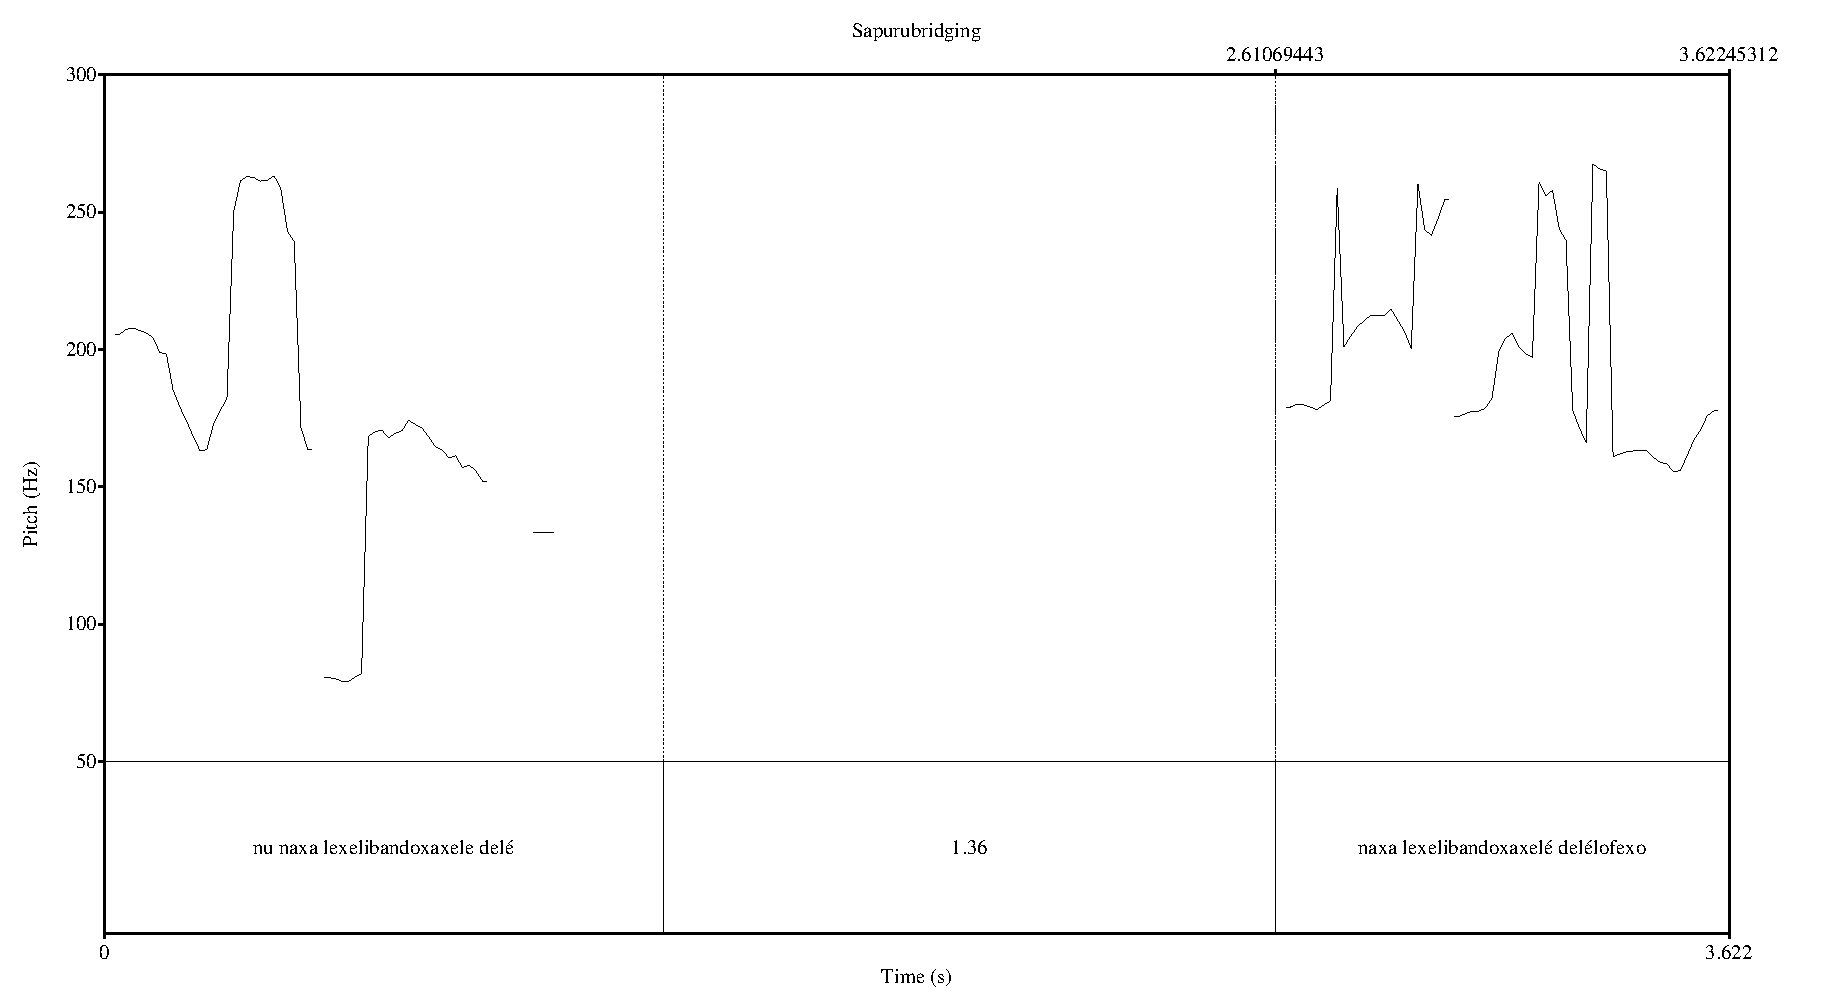
\includegraphics[width=\textwidth]{figures/devriesFig1.eps}
\caption{Intonation contour of example (\ref{Devex:10ab}) extracted with PRAAT. \label{DevF1}}
\end{figure}


The narrator, Sapuru, tells a real-life first person \isi{narrative} about how he tried to cut loose a captured person that his opponents wanted to kill and eat. In (\ref{Devex:10b}) he narrates what he told his opponents and in \REF{Devex:10b} the \isi{final clause} (with the quote-marking verb \textit{de} `to say') is repeated in the bridging clause, but now there is a \textsc{ds} \isi{conjunction} attached to the quote-marking verb, to indicate that what follows is the reply from the opponents (what they said). The bridging clause also includes the last clause of the quotation clause. 

The very fact that the chain-final reference clause is repeated in the initial clause of the next chain implies that the repeated information is now given and in this sense in the background, just as this is the case in \isi{recapitulative linkage} with thematic clauses (discussed in the next section). But the key difference between the two types of recapitulation is that the chained bridging clause is informationally and syntactically an ``online'' clause that presents given information, while thematic bridging clauses are ``offline'' background clauses. The on line nature of chained bridging clauses makes this linkage type one of \isi{thematic continuity}, both referentially through the continued \isi{switch reference} monitoring of topical participants and in terms of \isi{sequential} \isi{action} continuity (the \isi{event line}). 
	
	
\subsection{Recapitulative linkage with thematic clauses} 
\label{Devrecap.link.thematic}
This type is a less frequent type of \isi{recapitulative linkage} in which the bridging clause takes the form of a thematic clause, marked with the subordinator \textit{=xa} (and/or other subordinators), and optionally marked by the \isi{topic} marker \textit{=(f)efè}. It has two functions. The first function is the processual pause function that it shares with \isi{recapitulative linkage} with chained bridging clauses.

The second function is to present the repeated information as an \textit{offline} theme, a theme off the continuing event and participants line. The break in \isi{thematic continuity} with the preceding \isi{clause chain} is signaled by the discontinuation of \isi{switch reference} monitoring and the
obligatory presence of an independent verb form with \isi{TAM} specification that is not under the scope of the \isi{TAM} marking on the verb of the \isi{final clause}.  In contrast, a chained bridging clause presents the repeated clause as \textit{online} information integrated into the continuing event and  participant  lines. The chained bridging clause cannot be marked by a subordinator or the \isi{topic} marker \textit{=(f)efè}. The continuing event and participant lines are carried over the boundary  between two consecutive clause chains by obligatory \isi{switch reference} marking on the repeated verb in the chained bridging clause. In other words, chained bridging clauses form chaining paragraphs,  but thematic  bridging clauses disrupt and discontinue chaining paragraphs for various purposes, for example because the speaker wants to add important background information or wants to specify a reason why an event on the \isi{main event line} happened, as in (\ref{Devex:11b}). 

Thematic subordinate clauses in Greater Awyu languages behave like noun phrases, and they may take markers that also go with noun phrases to  express semantic or pragmatic relations, for example the general subordinator \textit{=xa}, the  reason marker \textit{lexé} that marks the bridging clause of (\ref{Devex:11b}) or the \isi{topic} marker \textit{=(f)efè}. It is this noun phrase characteristic that explains the association with disruption or ``going offline'' when thematic clauses are used as bridging clauses: the events they denote are not part of the \isi{main event line} expressed by chained clauses.

\begin{exe}
\ex \label{Devex:11ab}
\begin{xlist}
\ex \label{Devex:11a}		
\gll \textit{ü} \textit{dé=tofexo} \textit{a} \textit{gu} \textit{ü}	\textit{du-n-da} \textit{gu-pa} \textit{ü-axa-lé} \underline{\textit{dé}}\\
Ow!	say\textsc{[non1.sg.rls]=ds} ah you ow! say-\textsc{inf-neg} you-also kill-\textsc{irr-1sg} say\textsc{[non1.sg.rls]}\\
\glt `Ow, he\textsubscript{i} said and he\textsubscript{j} said, ah you must not say, ow, I will kill you also'\\

\ex \label{Devex:11b}		
\gll \textbf{\textit{dé=xa}} \textit{lexé} \textit{lenggilé=daxu} \textit{yaxatimexo}\\
say\textsc{[non1.sg.rls}]=\textsc{conn} cause be.frightened[\textsc{non1.sg.rls}]=\textsc{ss} renounce[\textsc{non1.sg.rls}]\\
\glt `Because he\textsubscript{j} said that, he\textsubscript{i} was afraid and renounced'\\
\end{xlist}
\end{exe}

Compare the \isi{recapitulative linkage} with thematic subordinate bridging in (\ref{Devex:11b}) and with chained bridging in (\ref{Devex:12b}), both involving the same verb of speaking \textit{de} `to say'. In (\ref{Devex:12b}) the verb of speaking of the reference clause is repeated in a chained \isi{switch reference} marked bridging clause, a bridging clause on the continuing \isi{event line}. But in (\ref{Devex:11b}) the same verb is repeated in a subordinate bridging clause, an offline clause that provides background information with regard to the \isi{event line}. The \isi{switch reference} monitoring of participants is carried across the boundary between (\ref{Devex:12a}) and (\ref{Devex:12b}). The chains (\ref{Devex:12a}) and (\ref{Devex:12b}) are chained into a \isi{chaining paragraph} in which \isi{switch reference} helps the listener to identify who is doing what from one sentence to the other. But this \isi{switch reference} monitoring is disrupted by the subordinate bridging clause of (\ref{Devex:11b}) and the listener has to identify the referents of the subjects solely on the basis of the context. 


\begin{exe}
\ex \label{Devex:12ab}
\begin{xlist}
\ex \label{Devex:12a}		
\gll \textit{le‑bo=to=fexo} \textit{nggé} \textit{nabul} \textit{nu} \textit{ne‑banun} \textit{bimo‑m} \underline{\textit{dé}}\\
come‑be[\textsc{non1.sg.rls}]=\textsc{ds}=\textsc{conn} friend brother.in.law \textsc{1sg} my‑back look‑\textsc{2sg.imp} say.\textsc{non1.sg.rls} \\
\glt `He came and said, Friend, brother-in-law, you must have a look at my back'\\

\ex \label{Devex:12b}		
\gll \textbf{\textit{dé=do}} \textit{a} \textit{ati} \textit{woxelimexo=do} \textit{ü} \textit{yi‑pa} \textit{xayo} \textit{baosa‑m‑b}o \textit{mé‑lai}\\          
Say[\textsc{non1.sg.rls}]=\textsc{ds} ah hold turn[\textsc{non1.sg.rls}]=\textsc{ds} ow \textsc{3sg}‑self  	arrow pierce‑do‑be[\textsc{non1.sg.rls}] move‑come[\textsc{non1.sg.rls}]\\
\glt `He said, and as they turned him around, Ow, my!, he had come pierced with arrows!'\\
\end{xlist}
\end{exe}

	
\section{Summary linkage} 
\label{Devsumm.link}
There are two types of \isi{summary linkage} of sentences. Both are used only occasionally. The first is with a \isi{demonstrative verb} \textit{(w)amo(l)-} `to do/to be that/thus/in that way' in a chained bridging clause, as in (\ref{Devex:16b}). The second type, rare in our texts, is with the same \isi{demonstrative verb} but now in a \textit{=xa} marked thematic clause, (\ref{Devex:18b}). The \isi{demonstrative verb} may also be used in other contexts as in (\ref{Devex:13}) and (\ref{Devex:14}).


\begin{exe}
\ex \label{Devex:13}
\gll \textit{yaxof-exa=lo} \textit{wof=exa} \textit{a-mo-mémo?}\\
who-\textsc{conn=foc} that=\textsc{conn} that-do-\textsc{imm[non1.sg.rls]}\\
\glt `Who just did that?'\\
\end{exe}
	     
\begin{exe}
\ex \label{Devex:14}
\gll \textit{mülalüp} \textit{nu-pa} \textit{amo-ba-lé}\\
formerly I-self do.thus-\textsc{pfv-1sg[rls]}\\
\glt `I myself have done things like that in former times'\\      	
\end{exe}

The \isi{demonstrative verb} \textit{(w)amo(l)-} is used both to link sentences and to link clauses within sentences (as in (\ref{Devex:15}), \textit{wa‑mo-nè}), but the latter use is much more frequent than the use as bridging clauses in \isi{summary linkage}, (\ref{Devex:16b}). For example, the \textsc{ss} medial form of the verb \textit{wamonè} is used to link clauses within the sentence in (\ref{Devex:15}):


\begin{exe}
\ex \label{Devex:15}	     
\gll \textit{dé=daxu=fexo} \textit{n‑até=lo} \textit{wa‑mo-nè} \textit{umo=do} \textit{dai‑ba‑lé}\\
say[\textsc{non1.sg.rls}]=\textsc{ss=conn} \textsc{1sg.poss}‑father=\textsc{foc} that-do-\textsc{ss}  		tell[\textsc{non1.sg.rls}]=\textsc{ds} hear‑\textsc{pfv‑1sg[rls]}\\
\glt `He told it to my father and likewise he (my father) told it and I listened.'\\	     
\end{exe}
	     
Example (\ref{Devex:16a}) gives just the last two clauses of a \isi{chaining paragraph} in directive mood, a prayer to the ancestors that accompanies a sacrifice \citep[see examples (8--22) in][160--162]{enk97}. It looks as if \textit{wamolmo} in (\ref{Devex:16b}) is used as a bridging clause that has the previous paragraph (the prayer as a whole, see \ref{Devex:07ae}) as its reference, summarizing and pointing back to it, rather than just the \isi{final clause} of the prayer episode. The quoted prayer in directive mood with second person verb forms ends in (\ref{Devex:16a}) and the narrator switches to third person subjects and to the habitual aspect in (\ref{Devex:16b}) with \isi{summary linkage} (`thus they always do') as the bridge between prayer and the continued narration.
	     
	     
\begin{exe}
\ex \label{Devex:16ab}
\begin{xlist}
\ex \label{Devex:16a}			     
\gll \textit{le‑mén=daxu}  \underline{\textit{noxu}} \underline{\textit{im-ba‑mon=è}}\\
eat‑\textsc{2pl.imp=ss} \textsc{1pl} see‑stay‑\textsc{2pl.imp=ex}\\
\glt `you must eat and keep taking care of us'\\
 
\ex \label{Devex:16b}			     
\gll \textbf{\textit{wa‑mol‑mo}} \textit{mamaf} \textit{bau}\\    
thus‑do-do.\textsc{hab[ss]} a.little sit[\textsc{non1.sg.rls}]\\	
\glt `They usually do like that and then after a little while...'\\
\end{xlist}
\end{exe}
		
In a \isi{summary linkage}, the use of the generic \isi{demonstrative verb} in the bridging clause allows speakers to point back in a vague  and general way to what preceded, leaving it to the addressee to infer what the scope of the anaphoric reference is, for example the \isi{final clause} of the previous chain, or the previous chain as a whole or even  a whole episode (a chain of imperative sentences),  as in this case where it points back to the whole prayer episode that precedes.

In the next example (\ref{Devex:17ab}), the generic \isi{demonstrative verb} seems to refer back to the \isi{final clause} of the previous \isi{clause chain}, although it can be taken to have the whole preceding \isi{clause chain} in its scope:
	
	
\begin{exe}
\ex \label{Devex:17ab}
\begin{xlist}
\ex \label{Devex:17a}			     
\gll \textit{gexenép} \textit{anè} \textit{xa‑mén=é} \textit{dé=do} \textit{él} \textit{de‑nè} \textit{xenè} \textit{lapangga=fexo} \textit{xai‑ba‑lè=do} \textit{pesau} 	\underline{\textit{maun=an}}	\underline{\textit{\smash{pesahu}}} \underline{\textit{lai}} \\
\textsc{2pl} \textsc{hort} go‑\textsc{2pl.imp=ex} say[\textsc{non1.sg.rls}]=\textsc{ds} yes say‑\textsc{ss}	next air.strip=\textsc{conn} live‑be‑\textsc{1pl.rls=ds} aeroplane river=\textsc{loc} aeroplane come[\textsc{non1.sg.rls}]\\
\glt `She told us to go (home) and we agreed and we waited at the airstrip until the plane landed on the river.'\\
 
\ex \label{Devex:17b}			     
\gll \textbf{\textit{amo=to=fexo}} \textit{noxu-peninggi} \textit{bando-ai} \textit{fe‑nè} \textit{fu=to=fexo} \\       
do[\textsc{non1.sg.rls}]=\textsc{ds=conn}	\textsc{1pl.poss}-evangelist bring-descend take‑\textsc{ss} put[\textsc{non1.sg.rls}]=\textsc{ds=conn}\\
\glt `It did so and he (=the pilot) brought our evangelist and...'\\
\end{xlist}
\end{exe}

Example (\ref{Devex:18b}) shows the use of the summary verb in a thematic bridging clause, the second subtype of \isi{summary linkage}. The narrator of (\ref{Devex:18ab}) had so far been denied tobacco, although he had tried to get tobacco from them in a friendly, teasing manner and the thematic bridging clause points back to that refusal. 


\begin{exe}
\ex \label{Devex:18ab}
\begin{xlist}
\ex \label{Devex:18a}			     
\gll \textit{a} \textit{noxup} \textit{xeyop} \textit{é‑fu‑ba‑lè=lo=fexo} \underline{\textit{sü‑lexé}} \underline{\textit{ne}} \underline{\textit{bu‑lelo‑ba‑lé}}\\
\textsc{ex} \textsc{1pl} house sleep‑make‑stay‑\textsc{1pl.rls=ds=conn} tobacco‑reason	\textsc{1sg} tease‑be‑stay-\textsc{1sg[rls]} \\ 
\glt `In the house we slept and I was teasing (them) for tobacco.'\\

\ex \label{Devex:18b}			     
\gll \textbf{\textit{amo‑xa‑tél=exa}} \textit{minya} \textit{alip=ta} \textit{alü‑xa‑léf-é} \textit{de‑ba‑lé}	 \\      		
do‑\textsc{irr‑2pl[rls]‑tr=conn}	fuel here=\textsc{loc} burn‑\textsc{irr‑1sg‑ex} \textbf{say-stay-\textsc{1sg[rls]}}  \\
\glt `If you do so, I will raise a fire here by means of petro­leum, I said'\\
\end{xlist}
\end{exe}

	
\section{Other ways to link sentences} 
\label{Devotherways}
Recapitulative linkage with chained bridging clauses is by far the most common device for connecting sentences in \ili{Korowai} \isi{narrative} texts but speakers may also use a small set of discourse conjunctions that occur mostly within sentences and mean something like `next' or `and'. These conjunctions (or verbs used as conjunctions) can be used also to connect sentences, for example \textit{(me)sé} `next' and \textit{xenè} `and'; `next'. The latter is a medial \textsc{ss} form of the verb of going that can be used both as a lexical verb `to go' and as a discourse \isi{conjunction} meaning `next'.  \textit{Xenè} may also precede a recapitulative bridging clause, as in (\ref{Devex:19b}). 

\begin{exe}
\ex \label{Devex:19ab}
\begin{xlist}
\ex \label{Devex:19a}			     
\gll \textit{Ye} \textit{loxté=do} \textit{walüp=ta} \textit{walüp=ta} \textit{maxaya} \textit{au‑pexo=do} \textit{wa=fexo} \textit{ye} \textit{xülo} \textit{ye} \textit{xe‑bo=fexo} \textit{gup=to} \textit{anè} \underline{\textit{da‑mo‑m=é}} \underline{\textit{dé}}\\
\textsc{3sg} go.away[\textsc{non1.sg.rls}]=\textsc{ds} half.way=\textsc{loc} half.way=\textsc{loc} maxaya.bat voice‑do[\textsc{non1.sg.rls}]=\textsc{ds} there=\textsc{conn} \textsc{3sg} upstream \textsc{3sg} go‑stay[\textsc{non1.sg.rls}]=\textsc{conn} you=\textsc{foc} \textsc{hort} hear‑do‑\textsc{2sg.imp=ex} say[\textsc{non1.sg.rls}]\\
\glt `He went away and halfway a maxaya‑bat squeaked and there he went upstream and he commanded (the bat), let me know.'\\

\ex \label{Devex:19b}			     
\gll \textit{xe‑nè} \textbf{\textit{da‑mo‑m=é}} \textbf{\textit{dé=do}} \textit{ye} \textit{loxté} \\        		
go‑\textsc{ss} hear‑do‑\textsc{2sg.imp=ex} say.\textsc{non1.sg.rls=ds} \textsc{3sg} go.away[\textsc{non1.sg.rls}]\\
\glt `And after he commanded, `you should let me know', he (the bat) went away.'\\ 
\end{xlist}
\end{exe}

The discourse \isi{conjunction} \textit{(me)sé} `next, and' connects (\ref{Devex:20a}) and (\ref{Devex:20b}):

\begin{exe}
\ex \label{Devex:20ab}
\begin{xlist}
\ex \label{Devex:20a}			     
\gll \textit{le‑mén=daxu} \textit{mano‑pa‑mon=é}\\
eat‑\textsc{2pl.imp =ss}	good-make‑\textsc{2pl.imp=ex}\\
\glt `You should  eat it and help (us)!'\\
	
\ex \label{Devex:20b}			     
\gll \textit{mesé} \textit{xobül=fexo} \textit{woto=fexa} \textit{fo} \textit{fe‑nè} \textit{fu‑ma‑té=daxu}\\
next leg=\textsc{conn} sacred.place=a.certain get get‑\textsc{ss} put‑\textsc{hab-non1.p[rls]=ss}\\
\glt `And then they usually take another leg and put it down on another sacred place, and..'\\
\end{xlist}
\end{exe}

\section{Conclusions} 
\label{DevConclusions}
Recapitulative linkage of the chained type is highly frequent in \ili{Korowai} \isi{narrative} and \isi{procedural texts}. It has three functions. First, a \isi{processual function}, to give the addressee the time to process the information of  the \isi{clause chain} just heard and to give the speaker the time to plan his or her following \isi{clause chain}. The \isi{processual function} is also clear from \isi{prosodic} patterns associated with recapitulative linkage.  Second, it creates chains of clause chains, chaining paragraphs or even chaining episodes.  The third function  is in the domain of participant \isi{cohesion}: to carry \isi{switch reference}  monitoring of participants across from one \isi{clause chain} to the next by chained \isi{recapitulative linkage}.  

In Papuan languages where \isi{recapitulative linkage} with chained clauses functions in similarly frequent ways in conditions of \isi{thematic continuity}, the absence of \isi{recapitulative linkage} is a signal of \isi{thematic discontinuity} in texts based on \isi{sequential} event lines \citep[][375]{devries.2005}.  For example, Reesink writes how Usan in ``paragraphing, then, makes use of a number of criteria, of which absence of tail-head linkage in \isi{narrative} material is a major one, albeit not a sufficient condition'' \citep[][332]{reesink87}. In Korafe the absence of \isi{recapitulative linkage} marks various forms of \isi{thematic discontinuity} such as shifts from speaker orientation to addressee orientation, shifts in time, scene, or character configuration \citep[][337, 363]{farr99}. This is also true for \ili{Korowai}. 

Recapitulative linkage of sentences with thematic clauses is a deviation from the default option, both formally and functionally, and associated with the disruption of \isi{switch reference} monitoring of participants and with going off the \isi{event line} to provide topical background information in relation to one or more events on the \isi{event line}. It shares the \isi{processual function} with the chained type of \isi{recapitulative linkage}. It also shares the givenness of the recapitulated bridging clause with chained bridging but now as part of an explicit, marked presentation of the given clause as offline background,  giving  the addressee a strong signal that the flow of the \isi{narrative} is disrupted for special purposes.

Summary linkage allows speakers to be more vague in terms of what the reference is of their anaphoric linkage with demonstrative-derived verbs. Summary linkage may refer back to the \isi{final clause} of the previous sentence, to the previous sentence as a whole or even to the preceding chain of sentences. This makes it useful in conditions of thematic re-orientation.

Both recapitulative and \isi{summary linkage} seem to be phenomena restricted in \ili{Korowai} to \isi{event line} based genres of texts where the chronology of the reported events is reflected in the order of the narration. 

Recapitulative and \isi{summary linkage} both involve non-main bridging clauses: \textsc{ss} clauses with medial verbs, \textsc{ss} or \textsc{ds} marked clauses with independent verbs and ``adverbial'' thematic clauses. Switch reference marked clauses with independent verbs are non-main clauses in the sense that, once they are integrated into the sentence by \isi{switch reference} clitcs, they cannot independently select tense, mood or modality: they depend on the verb of the \isi{final clause} of the chain for selection of these features.

Mixing of summary and \isi{recapitulative linkage} has not been found so far in \ili{Korowai} texts. Recapitulative linkage in the majority of cases implies verbatim \isi{repetition} of the reference clause(s). However, the only obligatorily repeated element is the verb of the reference clause. Omission of noun phrases, both core and peripheral arguments, occurs with some regularity, as is to be expected given the preference for minimal clauses with only a verb. Addition of nominal material to the bridging clause, elements that do not occur in the reference clause, is very rare.


\section*{Appendix}
 \setcounter{equation}{0}
 \exewidth{(A23)}
The \ili{Korowai} text of this appendix was recorded and transcribed by Rev. G.J. van Enk in Yaniruma in the early 1990s. It is part of a folder with unpublished \ili{Korowai} texts that Rev. G.J. van Enk gave me after his retirement from Papua. I use the text from the van Enk corpus numbered D.1.7 as an illustration of recapitulative linkages in \ili{Korowai}. It is a short but complete text. I have reglossed the text and deleted the name of the main character because it is a real life story about witchcraft, a very sensitive \isi{topic} in the \ili{Korowai} community. The narrator is Fenelun Molonggai who talks about an interrogation of a suspected witch (N.) during a witch trial.\\


\begin{exe}
\exi{(A1)} \label{Devex:App1}
\gll \textit{noxup} \textit{N.} \textit{ati-lame-lè=daxu} \textit{gup} \textit{fala=xo=lolo?} \textit{xe-nè} \textit{yanop} \textit{mé-bol} \textit{lé-lé-mba-tèl=exo=lo?} \underline{\textit{de-lè}}\\
\textsc{1pl}	N. hold-bind-\textsc{1pl[rls]=ss} \textsc{2sg} what=\textsc{q=foc}	go-\textsc{ss} person ground-hole.(grave) eat-eat-\textsc{hab-non1.pl=q=foc} say-\textsc{1pl[rls]}\\
\glt `We had caught and bound N. and  we said, what about you, did you use to go to burial places to eat people?'
\end{exe}

\begin{exe}
\exi{(A2)} \label{Devex:App2}
\gll \textit{\textbf{de-lè}=lo=fexo} \textit{él} \textit{yup} \textit{mündiyop=tanux} \textit{ye-mayox=fexo} \textit{yanop} \textit{mé-bol} \textit{xe-ba-tè} \textit{dé}\\
say-\textsc{1pl[rls]=ds=conn} yes \textsc{3sg} once=only \textsc{3sg}-companion=\textsc{conn} person ground-hole go-\textsc{pfv-non1.pl[rls]}			say[\textsc{rls.non1.sg}]\\
\glt `We said and, yes he had gone only once with his mates to a grave, he said.'
\end{exe}			
			

\begin{exe}
\exi{(A3)} \label{Devex:App3}			
\gll \textit{yo}	\textit{anè}	\textit{umo-m} \textit{de-lè=lo=fexo}	\textit{a} \textit{gülé} \textit{alümexon} \textit{alümexon=ta}	\textit{ye-mayox=fexo} \textit{yanop}	\textit{mé-bol} \underline{\textit{xa-tè}} \textit{dé}\\
\textsc{adh}	\textsc{adh}	tell-\textsc{imp.sg}	say-\textsc{1pl.rls=ds=conn}	\textsc{inj}	night full.moon full.moon=in \textsc{3sg}-companion=\textsc{conn}	person		ground-hole	go-\textsc{non1.pl[rls]}	say[\textsc{rls.non1.sg}]\\
\glt `Come on tell us, we said and, uh, on a clear moonlit night with full moon he and his companions had gone to a burial site, he said.'\\
\end{exe}			

\begin{exe}
\exi{(A4)} \label{Devex:App4}			
\gll \textit{\textbf{xa-tè}=to=fexo} \textit{yanop} \textit{laxül}	\textit{ye-lidop=tanux} \textit{faxte-nè} \textit{lu-falé-bo} \textit{dé}\\
go-\textsc{non1.pl[rls]=ds=conn}	person corpse \textsc{3sg}-one=only float-\textsc{ss}	come.up-appear-\textsc{pfv.non1.sg} say[\textsc{rls.non1.sg}]\\
\glt `They had gone and one corpse had floated up and had made an appearance, he said.'
\end{exe}			
			
\begin{exe}
\exi{(A5)} \label{Devex:App5}			
\gll \textit{Alo-bo=do=mpexo} \textit{maun} \textit{nenilfo-bo=do=mpexo} \textit{sendok=to=mpexo} \textit{ali-mi-méma-tè=fexo} \textit{yu} \textit{ali-féda-té=tofexo} \underline{\textit{\smash{gololo}}}.\\
stand.up-\textsc{pfv.non1.sg=ds=conn} fluid much-sit[\textsc{non1.sg}]=\textsc{ds=conn} spoon=\textsc{ins=conn}	scoop-drink-\textsc{imm-non1.pl[rls]=conn} \textsc{3sg} scoop-give-\textsc{non1.pl[rls]=ds} be.afraid[\textsc{non1.sg.rls}]\\
\glt `It (the corpse) stood up and there was much (corpse) fluid and they had just begun to scoop it up with a spoon and drink it and then they scooped it up for him to drink but he was afraid.'\\
\end{exe}			
	
\begin{exe}
\exi{(A6)} \label{Devex:App6}			
\gll \textit{\textbf{gololo}=to=fexo}	\textit{ati-ba-té=daxu}	\textit{ya-xaxolof=an} \textit{ali-mexe-té=do} \textit{me=do=mpexo} \textit{wasü} \textit{sendok=to=fexo} \textit{yanop} \textit{nén-ax} \textit{ali-mi-xami-baxa-ti=fexo} \textit{külmexe-té=daxu=fexo} \textit{yexenép} \textit{xa-un=ngga} \textit{lexe-mema-té=to=fexo} \textit{yanop} \textit{loxül} \textit{xau-meléai=do} \textit{yexenép} \textit{gilfa-té} \textit{dé}\\
be.afraid[\textsc{non1.sg.rls}]=\textsc{ds=conn} hold-\textsc{pfv-non1.pl=ss} \textsc{3sg.poss}-mouth=\textsc{loc} scoop-do-\textsc{non1.sg[rls]=ds} drink[\textsc{rls.non1.sg}]=\textsc{ds=conn} there spoon=\textsc{ins=conn}	person rotten-water scoop-drink-sit-\textsc{hod-non1.pl[rls]=conn} finished-\textsc{non1.pl[rls]=ss=conn} \textsc{3pl}	go-\textsc{inf=conn}	aim-\textsc{imm-non1.pl[rls]=ds=conn} person	corpse down-descend[\textsc{non1.sg.rls}]=\textsc{ds} \textsc{3sg} departed-\textsc{non1.pl[rls]} say[\textsc{rls.non1.sg}]\\
\glt `He was afraid and then they held him and scooped the corpse fluid into his mouth and he drank it and they were scooping  and drinking corpse fluid  there until they were done and then they wanted to go away and when the corpse had sunk, they left, he said.'\\		
\end{exe}						
			
			
			
\section*{Abbreviations}
\begin{multicols}{2}
\begin{tabbing}
\textsc{coord} \hspace{.5cm} \= second or third person\kill
\textsc{1}     \> first person (speaker)\\
\textsc{2}     \> second person\\
\textsc{adh}   \> adhortative\\
\textsc{caus}  \>  causative\\
\textsc{conn}  \>      connective\\
\textsc{coord} \>     coordinator\\
\textsc{ds}    \>    different subject\\
\textsc{emph}  \>      emphasis\\
\textsc{ex}    \>    exclamative\\
\textsc{foc}   \>     focus\\
\textsc{hab}   \>     habitual\\
\textsc{hod}   \>     hodiernal past\\
\textsc{hort}  \>      hortative\\
\textsc{imm}   \>     immediate\\
\textsc{imp}   \>     imperative\\
\textsc{inf}   \>     infinitve\\
\textsc{ins}   \>     instrument\\
\textsc{iter}  \>      iterative\\
\textsc{irr}   \>     irrealis\\
\textsc{loc}   \>     locative\\
\textsc{neg}   \>     negative\\
\textsc{non1}  \>      second or third person \\ \> (non-speaker)\\
\textsc{pfv}   \>     perfective\\
\textsc{pst}   \>     past\\
\textsc{pl}    \>    plural\\
\textsc{poss}  \>      possessive\\
\textsc{q}     \>     question marker\\
\textsc{rls}   \>     realis\\
\textsc{sg}    \>    singular\\
\textsc{ss}    \>    same subject\\
\textsc{top}   \>     topic\\
\textsc{tr}    \>    transitional sound\\
\textsc{voc}   \>     vocative
\end{tabbing}
\end{multicols}

\section*{Acknowledgements}
I would like to thank Valérie Guérin, Clemens Mayer, and two anonymous reviewers for their helpful critical comments.


\sloppy

\printbibliography[heading=subbibliography,notkeyword=this]
%{\sloppy
%\printbibliography[heading=subbibliography,notkeyword=this]
%}
\end{document}
